\documentclass{article}
\usepackage[utf8]{inputenc}
\usepackage{graphicx}
%Polski
\usepackage{polski}
\usepackage[utf8]{inputenc} 
%Kod
\usepackage{listings}
\usepackage{xcolor}
\usepackage{color}
\definecolor{codegreen}{rgb}{0,0,0}
\definecolor{codegray}{rgb}{0,0,0}
\definecolor{codepurple}{rgb}{100,0,0}
\definecolor{backcolour}{rgb}{255,255,255}

\lstdefinestyle{mystyle}{
    backgroundcolor=\color{backcolour},   
    commentstyle=\color{codegreen},
    keywordstyle=\color{magenta},
    numberstyle=\tiny\color{codegray},
    stringstyle=\color{codepurple},
    basicstyle=\ttfamily\footnotesize,
    breakatwhitespace=false,         
    breaklines=false,                 
    captionpos=b,                    
    keepspaces=true,                 
    numbers=none,                    
    numbersep=5pt,                  
    showspaces=false,                
    showstringspaces=false,
    showtabs=false,                  
    tabsize=2
}

\lstset {style=mystyle}

\title{Specyfikacja Implementacyjna}
\author{Ochnio Szymon i Sekula Sebastian}
\date{Marzec 2022}


\begin{document}
\maketitle

\section{Informacje ogólne}
Program będzie implementowany w języku "C", a do jego uruchomienia posłuży nam terminal linuxowy.
Program będzie w stanie generować graf składający się z węzłów według określonej wielkości kolumn oraz wierszy, a także przypisywać do krawędzi wagi z~określonego przedziału. Umożliwi również podział grafu na spójne podgrafy. Na główne zadania programu będzie składało się sprawdzenie spójności grafu przy pomocy algorytu BFS oraz znalezenienie najkrótszej ścieżki między dwoma zadanymi wierzchołkami za pomocą algorytmu Dijkstry.
\subsection{Flagi}
\begin{itemize}
    \item brak argumentów lub argumenty inne niż opisane poniżej - program wyświetla informację o niepoprawnej ilości argumentów i uruchamia podręcznego helpa.
    \item -h \textbar--help  \textbar-help \textbar-? - wyświetla podręcznego helpa
    \item -s source\_file [string] - nazwa pliku źródłowego (użycie tej flagi sprawia, że podanie wartości dla flag -x i -y nie będzie miało znaczenia, bo ilość wierszy oraz kolumn zostanie wczytana z pierwszej linii podanego pliku)
    \item -x x\_columns [int] - liczba kolumn węzłów w grafie. Wartość domyślna: 5.
    \item -y y\_rows [int] - liczba wierszy węzłów w grafie. Wartość domyślna: 5.
    \item -n n\_subgraphs [int] - pozwala podzielić graf na spójne i rozłączne względem siebie grafy. ${1 \leq n \leq (x*y)/2}$ (wielkość zmiennej domyślniej jest ustawiona na 1, graf nie jest dzielony na żadne podgrafy, wpisanie wartości mniejszej od 1 traktowane jest jako błąd). Flaga nie ma zastosowania w momencie, kiedy wczytany przez użytkownika graf jest niespójny, program da o tym znać stosownym komunikatem.
    \item -b begin\_node [int] - węzeł początkowy szukanej ścieżki. \newline [FLAGA OBOWIĄZKOWA]
    \item -e end\_node [int] - węzeł końcowy szukanej ścieżki. \newline [FLAGA OBOWIĄZKOWA]
    \item -r result\_file [string] - nazwa pliku docelowego
    \item -f from\_weight [double] - początek zakresu wag (włącznie). Wartość domyślna: 1.0 (kropka jako separator dziesiętny)
    \item -t to\_weight [double] - koniec zakresu wag (włącznie). Wartość domyślna: 10.0. (kropka jako separator dziesiętny)
    
\end{itemize}

\section{Zastosowane algorytmy}
\subsection{BFS (Breadth First Search)}
Algorytm wykorzystany do sprawdzania spójności grafu. \\
Działanie algorytmu:
\begin{enumerate}
    \item Zaczynamy w "zerowym" węźle i dodajemy wszystkie wierzchołki, które jesteśmy w stanie odwiedzić z zerowego wierzchołka do kolejki.
    \item Odwiedzając pierwszy węzeł z kolejki dodajemy wszystkich możliwych do odwiedzenia sąsiadów do kolejki ( nie wliczając węzła, który już został przez nas odwiedzony, ten możemy wrzucić do kolejki pomocniczej, która będzie zliczała odwiedzone węzły ).
    \item Idąc zgodnie z tym schematem przechodzimy przez całą nieustannie powiększającą się kolejkę, by na końcu sprawdzić, czy w kolejce zliczającej odwiedzone wierzchołki odwiedziliśmy wszystkie węzły, jeśli tak - graf jest spójny.

\end{enumerate}

\subsection{ Dijkstra } 
Algorytm Dijkstry wykorzystywany jest do znajdowania najkrótszej ścieżki w grafie łączącej 2 wierzchołki, przy czym nie działa on dla wag ujemnych. Przebieg algorytmu:
\begin{enumerate}
    \item Zainicjuj odległości do wszystkich wierzchołków jako nieskończone (DBL\_MAX) (tablica double distance[n]), tablicę z flagami czy dany wierzchołek był już odwiedzony wartościami 0 (tablica int seen[n]) oraz tablicę z numerem wierzchołka poprzedzającego, przez który prowadzi najkrótsza ścieżka  wartościami -1 (tablica int prev[n]).
    \item Stwórz pustą kolejkę priorytetową pq. Każdy element pq jest parą (waga, wierzchołek). Waga jest używana do porównywania par.
    \item Dodaj do kolejki parę (0, wierzcholek\_startowy)
    \item Dopóki kolejka nie będzie pusta lub nie zostanie osiągnięty wierzchołek końcowy wykonuj:
        \begin{enumerate}
            \item Weź z kolejki parę o najmniejszej wadze. Niech wzięty wierzchołek ma id = u.
            \item Przejdź po wszystkich nieodwiedzonych wierzchołkach sąsiadujących z u oznaczanych jako v:
            \begin{enumerate}
                \item Jeżeli distance[v] \textgreater (distance[u] + waga(u, v)) to:
                distance[v] = (distance[u] + waga(u, v)) oraz dodaj parę (distance[v], v) do kolejki priorytetowej
                \item Ustaw prev[v] = u
                \item Ustaw seen[v] = 1 
            \end{enumerate}
        \end{enumerate}
    \item Jeżeli droga do zadanego wierzchołka jest mniejsza od nieskończoności wypisz długość najkrótszej ścieżki i wierzchołki, przez które ona prowadzi, a w przeciwnym wypadku wypisz informacje że nie ma ścieżki łączącej zadane wierzchołki. 
\end{enumerate}

\section{Podział na moduły}
\begin{itemize}
\item queue.c, queue.h - moduł kolejki
\item priority\_queue.c, priority\_queue.h - moduł kolejki priorytetowej
\item graph.c, graph.h - moduł listy sąsiedztwa i generatora grafu
\item bfs.c, bfs.h - moduł algorytmu BFS
\item dijkstra.c, dijkstra.h - moduł algorytmu dijkstry
\item splitter.c, splitter.h - moduł algorytmu dzielącego graf na podgrafy
\item reader.c, reader.h - moduł algorytmu czytającego z pliku
\item writer.c, writer.h - moduł odpowiedzialny za zapis grafu do pliku
\item main.c - moduł główny, odpowiedzialny za przebieg programu
\item const.h - moduł przechowujący define'y
\end{itemize}

{\centering{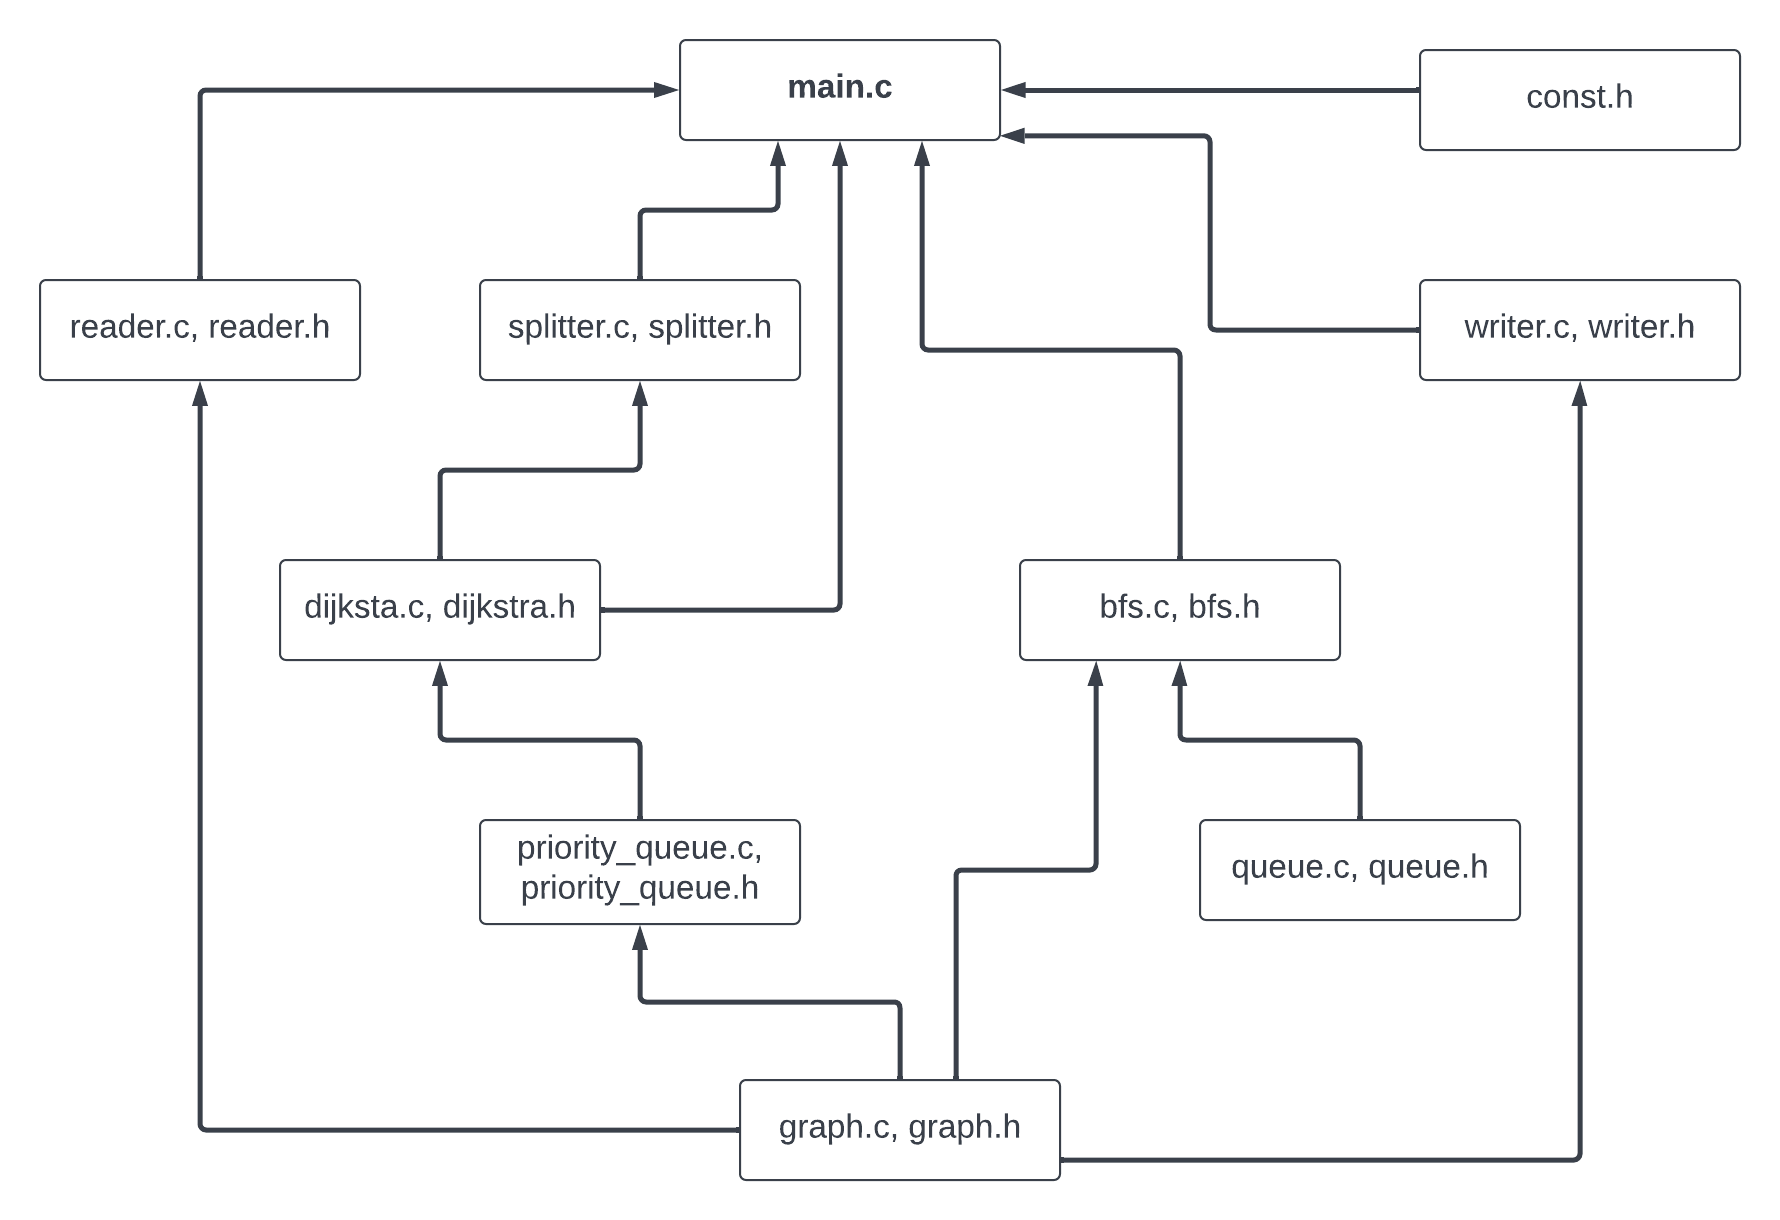
\includegraphics[scale=0.5]{diagram.png}} \\ }




\section{Struktury danych}
\subsection{Kolejka FIFO}
Jest to struktura, która przechowuje dane. Jako, że nasza kolejka jest kolejką FIFO ( First In First Out), znaczy to, że pierwszy umieszczony w niej element, będzie zarazem pierwszym elementem, który z niej wyjdzie jeśli tego zażądamy.
\\
Struktura ta znajdzie zastosowanie przy implementacji algorytmu BFS, gdzie każdy nowo napotkany wierzchołek będzie w niej umieszczany, a po jego odwiedzeniu - wyrzucany.
\subsection{Kolejka Priorytetowa}
Jest to struktura, która przechowuje dane. Ten specjalny rodzaj kolejki charakteryzuje się tym, że przy każdym włożeniu elementu do tej struktury, cała zawartość kolejki jest sortowana według priorytetu, sprawiając w ten sposób, że elementami, które jako opuszczą naszą strukturę będą te o największym priorytecie.
\\
Struktura ta będzie wykorzystywana w algorytmie Djiksry.
\subsection{Struktura przechowująca kolejkę priorytetową - pq\_t}
Kolejka będzie przechowywana w postacji tablicy typu pair\_t.
Ponadto znajdą się tu 2 pola typu int: size i capacity, przechowujące odpowiednio aktualny rozmiar kolejki i jej maksymalną pojemność.

%\subsection{Lista}
%Jest to struktura umożliwiająca przechowywanie danych. Charakteryzuje się tym, że nie podlega odgórnym ograniczeniom tak jak standardowe tablice, ta może być powiększana tak bardzo jak system na to pozwoli. Składa się ona ze struktur, które poza swoją zawartością, trzymają również wskaźnik na następny element listy.
\subsection{Struktura przechowująca listę sąsiedztwa - graph\_t}
Graf będzie przechowywany w liście sąsiedztwa w postaci tablicy dwuwymiarowej struktur typu pair\_t o rozmiarze n x 4, gdzie:
\begin{itemize}
\item n - liczba węzłów w grafie.
\item 4 - drugi wymiar tablicy, składający się z 4 stuktur typu "pair\_t"
\end{itemize}
Ponadto znajdą się tu 2 pola typu int: rows i cols przechowujące odpowiednio liczbę wierszy i kolumn w grafie
\subsection{Struktura przechowująca pary (waga, wierzcholek) - pair\_t}
Struktura, która przechowuje dwie wartości: double i int - odpowiednio wagę przejścia i numer wierzchołka. Jest ona podstawą tablicy przechowującej listę sąsiedztwa. Jest wykorzystywana także w kolejce priorytetowej. 
\section{Scenariusz Działania Programu}

\subsection{Scenariusz ogólny}
Program po uruchomieniu sprawdza poprawność podanych argumentów. 
\\
Jeżeli zostanie podany plik źródłowy, sprawdzana jest spójność grafu wejściowego przy pomocy algorytmu BFS. Jeżeli graf jest niespójny nie istnieje możliwość podzielenia go na więcej podgrafów, w przeciwnym wypadku następuje podział na n podgrafów.
\\
Jeżeli plik wejściowy nie zostanie podany, następuje wygenerowanie grafu według zadanych parametrów.
\\
W dalszym ciągu program szuka przy pomocy algorytmu Dijkstry najkrótszej ścieżki dla zadanych dwóch wierzchołków wyświetla jej długość i przebieg lub informację o jej braku (np. gdy wskazane wierzchołki znajdują się w oddzielnych podgrafach).
\\
W dalszej kolejności ewentualnie przekształcony graf jest zapisywany do pliku lub wypisywany na standardowe wyjście.

\subsection{Scenariusz szczegółowy}
\begin{enumerate}

\item Czy została podana flaga -s ?
    \begin{itemize}
        \item Tak - Czy udało się wczytać source\_file?
        \begin{itemize}
            \item Tak - Następuje wczytanie grafu z podanego pliku do programu. Flagi -x i -y zostaną zignorowane.
            \item Nie - program wyświetla komunikat o błędzie i kończy swoje działanie.
        \end{itemize}
        \item Nie - Graf jest generowany według podanych -x, -y, -n i zakresu wag.
    \end{itemize}
    
\item Program sprawdza czy wczytany graf jest spójny przy pomocy algorytmu BFS.

\item Czy została podana flaga -n ?
    \begin{itemize}
        \item Tak - jeśli graf jest spójny następuje podział grafu na wskazaną liczbę podgrafów. W przypadku, kiedy graf nie jest spójny następuje informacja o tym, że nie można podzielić tego grafu na wskazaną liczbę podgrafów.
    \end{itemize}

\item Czy zostały wykorzystane flagi -b -e ?
    \begin{itemize}
        \item Tak - program przy użyciu algorytmu Dijkstry znajdzie najkrótszą ścieżkę między podanymi wierzchołkami, wypisze jej długość i pokaże przebieg.
        \item Nie - program wyświetla komunikat o błędzie i kończy swoje działanie.
    \end{itemize}

\item Czy została podana flaga -r ?
    \begin{itemize}
        \item Tak - graf zostaje zapisany do pliku o podanej nazwie w postaci listy sąsiedztwa.
        \item Nie - graf zostaje wypisany na standardowe wyjście.
    \end{itemize}
    
\end{enumerate}

%do szczególniejszego opisu
\section{Opis testów programu}
Wszystkie poniżej wymienione testy będą dostępne z poziomu Makefile'a w folderze projektowym. 
\begin{enumerate}
    \item make test1: Reakcja na niepoprawne parametry wywołania.
    \item make test2: Wczytywanie danych i reakcji na zły format danych w pliku.
    \item make test3: Definiowanie przez program grafu spójnego oraz niespójnego.
    \item make test4: Sprawdzanie przez program spójności grafu.
    \item make test5: Sprawdzanie czy istnieje ścieżka pomiędzy podanymi wierzchołkami.
    \item make test6: Liczenie najkrótszej ścieżki między podanymi wierzchołkami.
    \item make test7: Wskazywanie przebiegu najkrótszej ścieżki.
    \item make test8: Wypisywanie grafu na wyjście.
\end{enumerate}
Wszystkie poprawne wyniki wywołań poszczególnych testów znajdują sie w pliku "testy.txt", znajdującym się w folderze projektowym.
\\
Poza wymienionymi wyżej funkcjami użytkownik przy wpisaniu komendy "make" skompiluje cały kod tworząc plik wynonywalny.
\\
Dostępna jest również komenda "make test", która uruchomi wszystkie 8 wyżej wymienionych testów za jednym razem. 
\\

\end{document}
